\section{Linial's Algorithm}

We now give the description of an algorithm that can be used to merge under
partial information. The merging under partial information problem is the
following,

\begin{problem}
Given a poset \(P\) that can be covered by two chains \(A\) and \(B\), find a
linear extension of \(P\).
\end{problem}

\begin{figure}
\centering
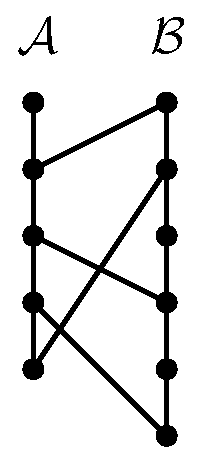
\includegraphics[height=0.2\textheight]{fig/supi/mupi}
\caption{A poset \(P\) covered by two chains \(A\) and \(B\),
input of the MUPI problem.}
\label{fig:supi:mupi}
\end{figure}

\citet*{linial:1984} first proves that the \onethirdtwothird conjecture holds
for width-\(2\) posets, \ie posets that can be covered by two chains. Since one
can always find a good query in \(P\) that when answered will invalidate at
least one third of the possible linear extensions, it is possible to design a
\BigO{\log e(P)} algorithm that solves the MUPI problem.

\begin{theorem}
Given a poset \(P\) covered by two chains \(A\) and \(B\), we can always find
a query \(x \ask{\le} y\) with \(x \in A, y \in B\) such that the probability
that \(x \le y\) lies in the interval \([\sfrac{1}{3}, \sfrac{2}{3}]\).
\end{theorem}

\citet*{linial:1984} proposes the following algorithm. We compute the number of
linear extensions of the width-\(2\) poset \(P\) using the determinant
counting formula. The proof for this determinant counting formula can be found in
\citet*{mohanty:1979}, we give hereunder the statement of this formula in the
context of the merging under partial information problem.

\begin{theorem}
Let \(P = A \cup B\), where \(A = (\chain{a_1}{a_m})\) and \(B =
(\chain{b_1}{b_n})\), and assume \(m \ge n\). Define the integers
\(\alpha_1,\ldots,\alpha_m,\beta_1,\ldots,\beta_m\) as follows, \(\beta_i =
min\{t \st b_t > a_i\}, \alpha_j = max\{t \st b_t < a_j\}\) and where the
minimum and maximum of an empty set are taken to be \(n + 1\) and \(0\)
respectively. The number of extensions of \(P\) is given by

\begin{displaymath}
e(P) =
\begin{vmatrix}
\binom{\beta_i - \alpha_j}{j - i - 1}_{+}
\end{vmatrix}_{1 \le i , j \le m},
\end{displaymath}

the determinant of a \(m \times m\) matrix. The special \(\binom{n}{k}_{+}\)
notation is defined by

\begin{displaymath}
\binom{n}{k}_{+} =
\begin{dcases*}
0            & if  \(n < 0\)  or \(k < 0\)  or \(k > n\)\\
1            & if \(k = 0\)  or \(k = n\)\\
\binom{n}{k} & otherwise\\
\end{dcases*}.
\end{displaymath}
\end{theorem}


